\chapter{HASIL DAN PEMBAHASAN}
Pada subbab pertama pada bab ini akan dipaparkan hasil akhir dari pengerjaan tugas akhir Interoperabilitas NFT Berbasis \emph{Blockchain} Menggunakan \emph{Smart Contract} pada WEB3.0. Pada subbab selanjutnya akan dipaparkan mengenai hasil pengujian dari hasil tugas akhir untuk memastikan bahwa sistem yang dikembangkan berjalan dengan sesuai.

\section{Hasil}
Hasil keseluruhan dari sistem yang dikembangkan adalah \emph{interface} berupa web, \emph{Non-Fungible Token} (NFT) dan juga \emph{smart contract} yang berinteroperabilitas. Berikut dipaparkan masing-masing hasil dari sistem yang dikembangkan.

\section{Pengujian}
Untuk memastikan bahwa sistem interoperabilitas \emph{Smart Contract} berjalan sesuai dengan yang direncakan maka perlu dilakukan pengujian lebih lanjut. Pengujian yang dilakukan secara garis besar dibagi menjadi dua yaitu pengujian fitur-fitur utama dari \emph{Smart Contract} yang meliputi \emph{minting}, dan transfer \emph{ownership} kepemilikan NFT dan yang kedua adalah pengujian integrasi ke \emph{interface} yang telah dibuat. Masing - masing dari pengujian akan dibagi menjadi 3 sub bab:

\begin{enumerate}[nolistsep]
\item Yang pertama pada \ref*{sec:pengujian_pertama} terdapat Pengujian \emph{Smart Contract}
\item Yang kedua pada \ref*{sec:pengujian_kedua} terdapat Hasil Pengujian \emph{Minting} NFT
\item Lalu pada \ref*{sec:pengujian_ketiga} Hasil Pengujian Transfer \emph{Ownership}.
\end{enumerate} 

\subsection{Pengujian \emph{Smart Contract}}
\label{sec:pengujian_pertama}
Ekspektasi pengujian dari sistem \emph{smart contract} antara lain adalah sebagai berikut:
\begin{itemize}
    \item \emph{User} dapat melakukan minting token NFT yang kemudian kepemilikan NFT tersebut dapat dilihat pada \emph{test net} \emph{platform} OpenSea.

    \item Antar \emph{user} yang berbeda \emph{Network} dapat saling berkomunikasi dan kepemilikan \emph{token} NFT dapat berpindah dari \emph{user} A yang berada pada \emph{network} A' ke \emph{user} B yang berada pada \emph{network} B'.
\end{itemize}

Dalam penelitian ini, dilakukan pengujian interoperabilitas dan transfer ownership NFT menggunakan dua skenario berbeda yang dicatat dalam dua tabel. Tabel pertama, yang tercantum sebagai "Informasi Akun Testing Beda Network," digunakan untuk menguji kemampuan smart contract dalam mengirimkan NFT antar dua jaringan blockchain yang berbeda dari Sepolia Ethereum Testnet ke BNB Chain Testnet. Setiap akun diwakili oleh alamat unik yang beroperasi di network yang telah ditentukan, memungkinkan pengujian transfer aset digital lintas lingkungan blockchain yang berbeda. 

\begin{center}
\begin{table}[H]
      \centering
      \caption{Informasi Akun Testing Beda \emph{Network}}
      \begin{tabular}{|c|c|c|}
      \hline
      \textbf{Akun} & \textbf{Address} & \textbf{\emph{Network}}
      \\
      \hline
      A & 0x6A1B77e82b61D54C4F1A27cd00A27325EBf361eD & \emph{Sepolia Ethereum Testnet}
      \\ 
      \hline
      B & 0xD066d6576D9485Eb2c2a41BB8B52EcE17a0557d6 & \emph{BNB Chain Testnet} \\
      \hline
      \end{tabular}      
      \label{tab:akun_beda_multiple_network}
\end{table}
\end{center}

\begin{center}
  \begin{table}[H]
        \centering
        \caption{Informasi Akun Testing Sesama \emph{Network}}
        \begin{tabular}{|c|c|c|}
        \hline
        \textbf{Akun} & \textbf{Address} & \textbf{\emph{Network}}
        \\
        \hline
        Pertama & 0xf39Fd6e51aad88F6F4ce6aB8827279cffFb92266 & \emph{Localhost}
        \\ 
        \hline
        Kedua & 0x70997970C51812dc3A010C7d01b50e0d17dc79C8 & \emph{Localhost} \\
        \hline
        Ketiga & 0x3C44CdDdB6a900fa2b585dd299e03d12FA4293BC & \emph{Localhost} \\
        \hline
        \end{tabular}      
        \label{tab:akun_localhost}
  \end{table}
  \end{center}
  
  Sementara itu, tabel kedua, "Informasi Akun Testing Sesama Network," berfokus pada pengujian internal dalam satu jaringan, yaitu Localhost. Pengujian ini melibatkan beberapa akun yang berinteraksi dalam satu jaringan yang sama untuk mengevaluasi proses transfer ownership NFT antar akun dalam satu ekosistem yang sama.

  Berikut merupakan langkah-langkah dari pengujian sistem \emph{smart contract} yang akan dilakukan:

\begin{itemize}
    \begin{figure} [H] \centering
    % Nama dari file gambar yang diinputkan
    \emph{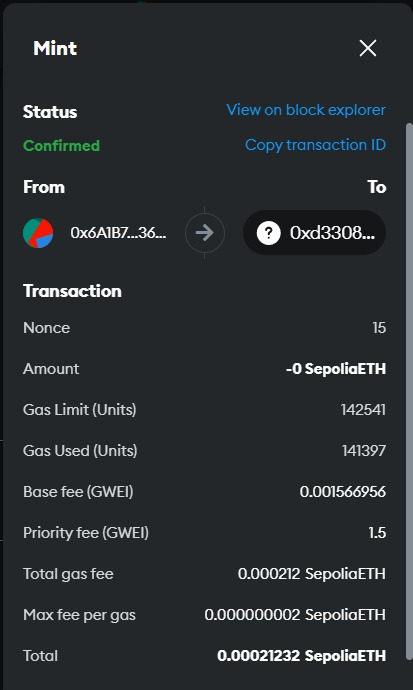
\includegraphics[scale=0.35]{gambar/riwayat_transaksi.jpeg}}
    % Keterangan gambar yang diinputkan
    \caption{Riwayat transaksi minting pada Metamask Wallet}
    % Label referensi dari gambar yang diinputkan
    \label{fig:minting}
    \end{figure}

    \item \emph{User} A akan melakukan \emph{minting} pada NFT dengan menggunakan MetaMask wallet, yang terhubung langsung ke Ethereum \emph{blockchain} melalui jaringan \emph{Sepolia Testnet}. Transaksi \emph{minting} ini mengkonfirmasi kreasi token baru di \emph{blockchain}, yang dicatat dengan detail transaksi seperti nonce, gas limit, dan biaya transaksi yang terdiri dari base fee dan priority fee. Proses ini mencatat NFT sebagai aset digital yang unik di \emph{blockchain}, memberikan hak kepemilikan digital kepada User A. Transaksi semacam ini memastikan keamanan dan transparansi dalam pencatatan kepemilikan aset digital, sekaligus mengintegrasikan NFT ke dalam ekosistem yang lebih luas di mana aset ini dapat diperdagangkan atau digunakan dalam aplikasi lain di masa depan.


    \item Tambahan dari gambar \ref*{fig:detail_transaksi_etherscan}, detail pada Etherscan memperlihatkan informasi kunci dari transaksi NFT yang dilakukan. \emph{Transaction hash} yang ditampilkan berfungsi sebagai pengenal unik transaksi, menunjukkan keberhasilannya pada \emph{blockchain}. Tanggal dan waktu transaksi juga tercatat, memberikan data penting mengenai kapan transaksi tersebut terjadi. Token yang terlibat adalah tipe ERC-721, standar untuk NFT yang memungkinkan representasi unik aset digital di Ethereum. Transaksi ini mencerminkan proses \emph{minting}, di mana NFT baru dibuat dan terdaftar di \emph{blockchain}, dan kemudian dialihkan dari alamat nol (menunjukkan penciptaan) ke alamat pemilik baru, yang dalam kasus ini adalah akun pertama yang melakukan \emph{minting}. Selain itu, biaya transaksi atau \emph{gas fee} yang relatif rendah menandakan efisiensi dalam pemrosesan transaksi tersebut di jaringan.

    \begin{figure} [H] \centering
    % Nama dari file gambar yang diinputkan
    \frame{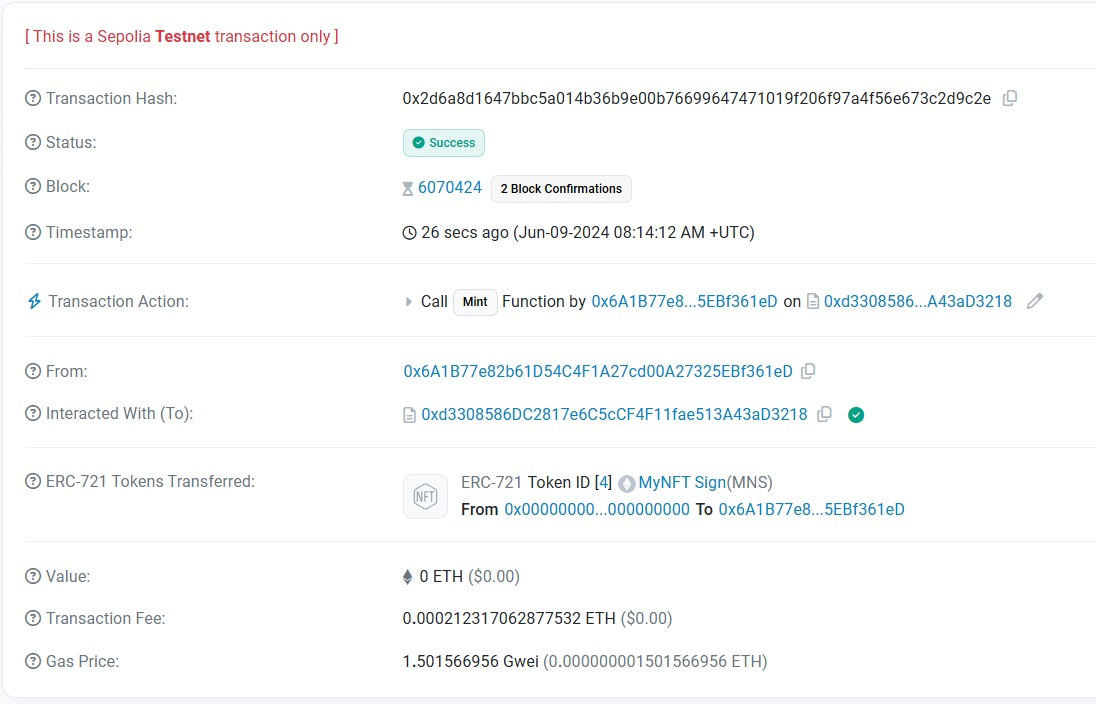
\includegraphics[scale=0.32]{gambar/detail_transaksi_etherscan.jpeg}}
    % Keterangan gambar yang diinputkan
    \caption{Detail transaksi pada Etherscan}
    % Label referensi dari gambar yang diinputkan
    \label{fig:detail_transaksi_etherscan}
    \end{figure}

    \item Pada gambar \ref*{fig:detail_nft_etherscan}, detail lebih lanjut mengenai NFT yang telah di-\emph{mint} juga dapat dilihat di Etherscan, seperti yang ditampilkan dalam gambar terlampir. Halaman Etherscan ini menyediakan data menyeluruh tentang NFT tersebut, termasuk alamat pemilik, alamat kontrak, dan pembuatnya. Setiap aspek dicatat dengan presisi untuk memastikan transparansi dan kemampuan dilacak dalam jaringan blockchain. Secara khusus, NFT ini, yang diidentifikasi sebagai "MyNFT Sign \#4", ditampilkan dengan ID token uniknya dan memastikan kepatuhan pada standar token ERC-721, yang menegaskan sifat non-fungible-nya. Tingkat detail ini penting untuk memverifikasi keaslian dan riwayat kepemilikan aset digital, membuat platform seperti Etherscan menjadi alat yang tak tergantikan dalam pengelolaan dan pertukaran NFT. Alat-alat ini juga meningkatkan keamanan transaksi digital dengan menyediakan jejak audit yang dapat diandalkan untuk setiap aset.

    \begin{figure} [H] \centering
    % Nama dari file gambar yang diinputkan
    \frame{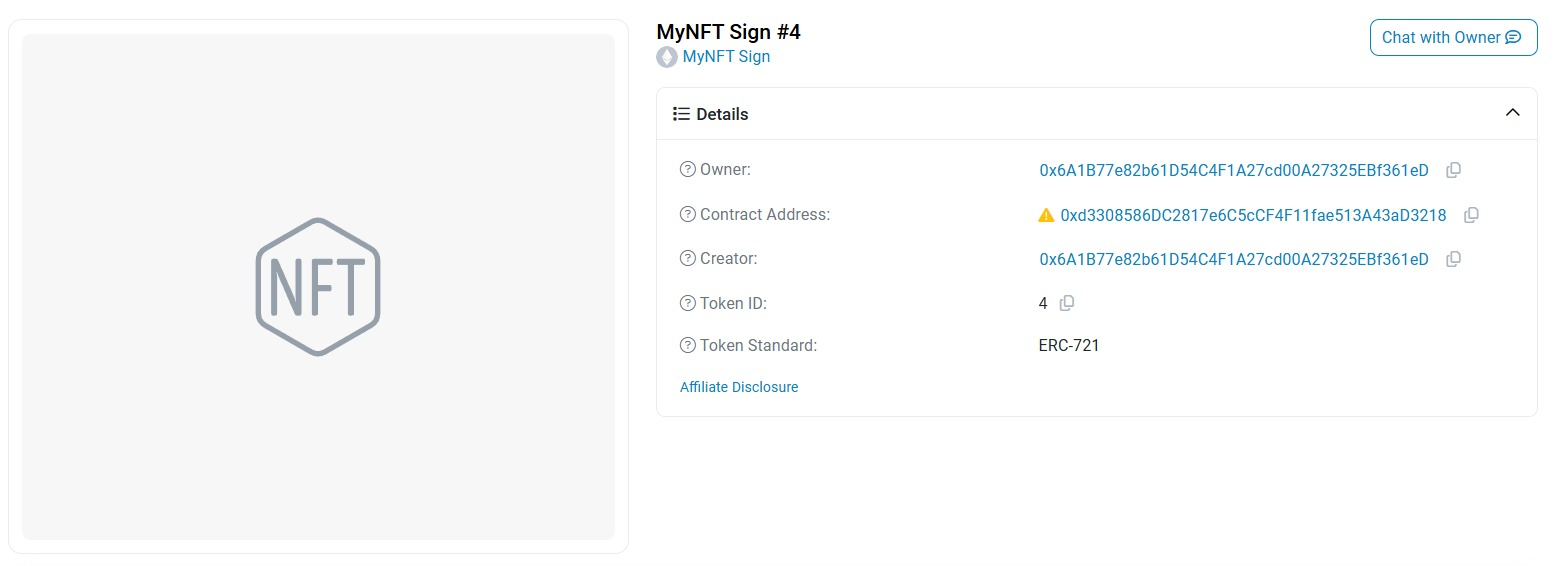
\includegraphics[scale=0.3]{gambar/detail_nft_etherscan.jpeg}}
    % Keterangan gambar yang diinputkan
    \caption{Detail NFT pada Etherscan}
    % Label referensi dari gambar yang diinputkan
    \label{fig:detail_nft_etherscan}
    \end{figure}
    
    \begin{figure} [H] \centering
    % Nama dari file gambar yang diinputkan
    \frame{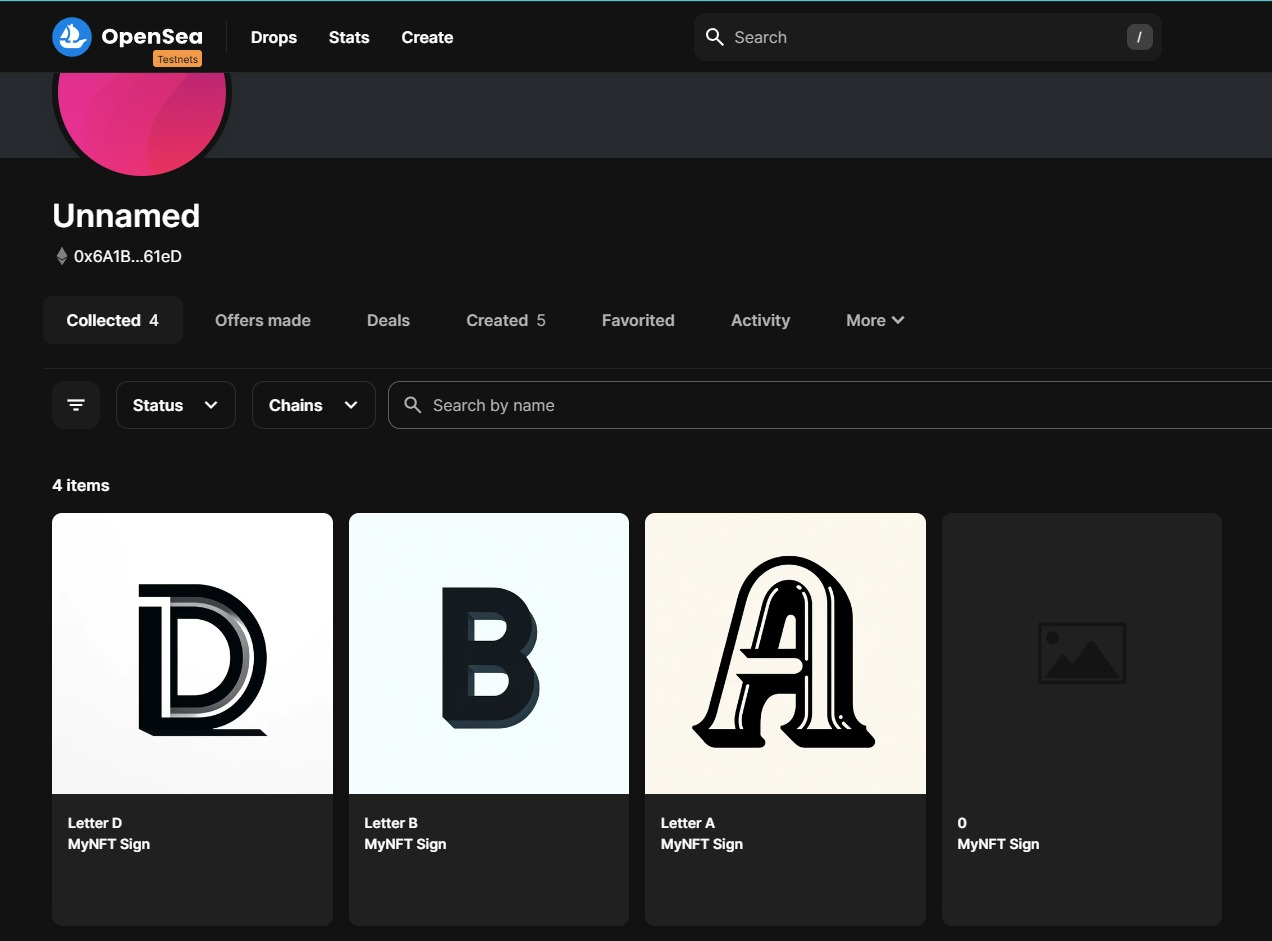
\includegraphics[scale=0.30]{gambar/nft_pada_opensea.jpeg}}
    % Keterangan gambar yang diinputkan
    \caption{NFT pada OpenSea}
    % Label referensi dari gambar yang diinputkan
    \label{fig:nft_opensea}
    \end{figure}

    \item Setelah proses \emph{minting} berhasil, seperti pada gambar \ref*{fig:nft_opensea} NFT yang telah di-\emph{minting} dapat dilihat pada platform OpenSea, yang merupakan pasar digital untuk aset kripto dan NFT. Dalam kasus pengujian ini, NFT yang telah di-minting adalah "Letter D", ditampilkan bersama dengan NFT lainnya yang telah dibuat oleh pengguna yang sama. Halaman OpenSea menampilkan berbagai detail seperti nama NFT, gambar, dan informasi lain yang relevan. Pengguna dapat melihat koleksi lengkap yang telah mereka mint atau beli. Setiap NFT ditampilkan dengan \emph{thumbnail} yang jelas, dan ketika di-klik, pengguna dapat melihat detail lebih lanjut seperti riwayat transaksi dan keaslian NFT tersebut. Ini memungkinkan pengguna untuk tidak hanya melihat koleksi mereka tetapi juga untuk berinteraksi dengan pasar, membuat penawaran, atau menjual NFT mereka.


    \item setelah NFT sudah terbuat, maka tahap berikutnya adalah melakukan \emph{lock} pada NFT yang akan dikirimkan ke \emph{user} B pada \emph{network} B'. Fungsi dari \emph{lock} ini untuk menjamin bahwa data token tidak diubah selama proses \emph{transfer}, menjaga kepercayaan dan keautentikan data NFT. Kemudian juga berguna untuk memberi sinyal kepada semua pihak terkait (pengguna, \emph{smart contract} di jaringan lain) bahwa token tersebut sedang dalam proses \emph{transfer}, dan operasi pada token harus ditangguhkan hingga proses selesai.

    \begin{figure} [H] \centering
    % Nama dari file gambar yang diinputkan
    \frame{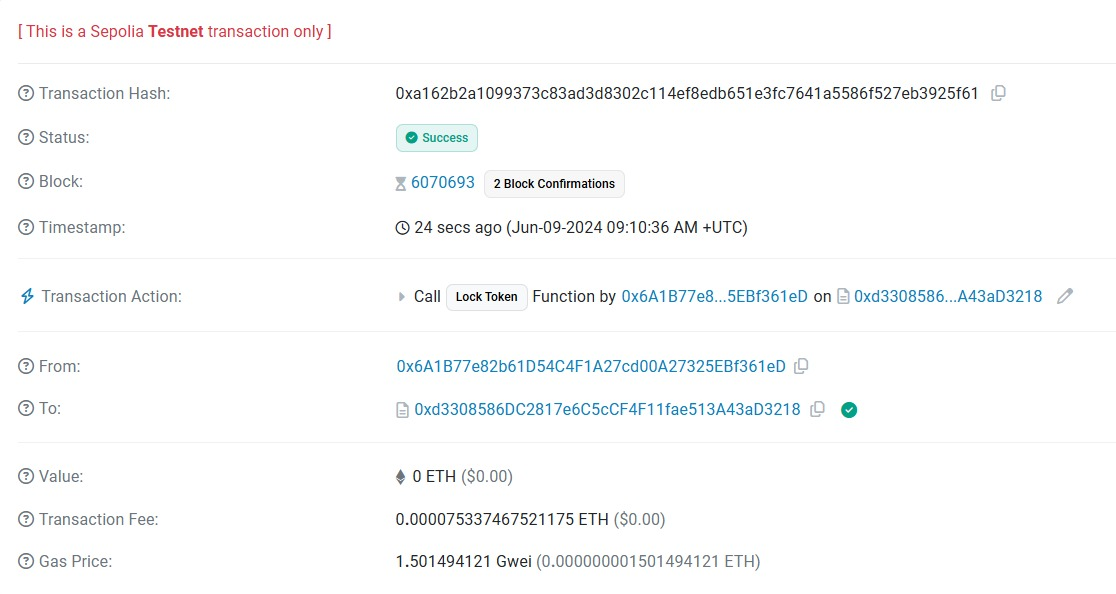
\includegraphics[scale=0.35]{gambar/lock_token.jpeg}}
    % Keterangan gambar yang diinputkan
    \caption{Detail fungsi \emph{Lock Token} pada Etherscan}
    % Label referensi dari gambar yang diinputkan
    \label{fig:locktoken}
    \end{figure}

    \item selesai melakukan proses \emph{lock token}, lalu fungsi \emph{bridge transfer} dapat dilaksanakan. Fungsi ini memfasilitasi transfer aman NFT antar \emph{blockchain} dengan memastikan bahwa NFT tersebut terkunci selama proses transfer dan memberikan visibilitas transparan tentang kejadian transfer melalui \emph{event} yang dicatat. Ini adalah komponen kunci dalam membangun aplikasi \emph{interoperable} yang memungkinkan aset \emph{digital} bergerak lintas ekosistem \emph{blockchain}.

    \begin{figure} [H] \centering
    % Nama dari file gambar yang diinputkan
    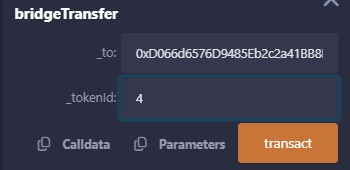
\includegraphics[scale=0.75]{gambar/bridge_transfer.jpeg}
    % Keterangan gambar yang diinputkan
    \caption{Parameter \emph{bridge transfer}}
    % Label referensi dari gambar yang diinputkan
    \label{fig:bridge_tranfer}
    \end{figure}

    \item pada gambar \ref{fig:bridge_tranfer} terdapat 2 parameter yaitu \texttt{"\emph{\_to}"}" yang digunakan untuk menerima parameter \emph{address} dari \emph{user} B dan juga parameter \texttt{"\emph{\_tokenId}"} untuk menerima argumen dari token NFT. Setelah dilakukan \emph{transact} maka akan dilanjutkan ke pembayaran pada Metamask Wallet.

    \begin{figure} [H] \centering
    % Nama dari file gambar yang diinputkan
    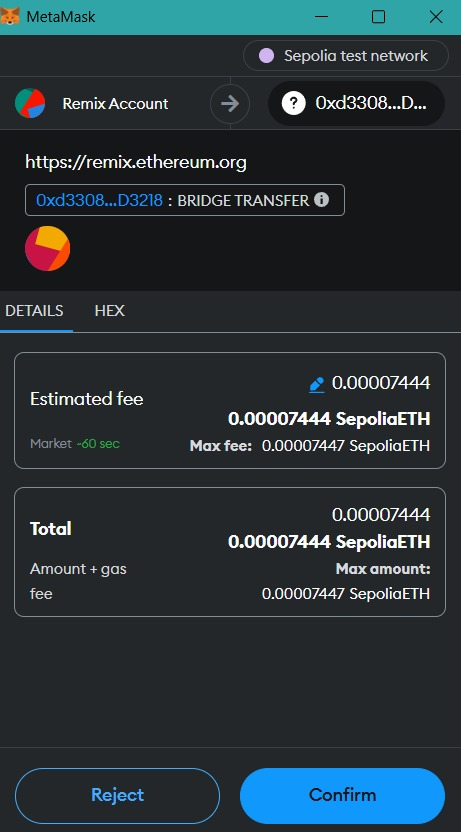
\includegraphics[scale=0.38]{gambar/verifikasi_metamask_wallet.jpeg}
    % Keterangan gambar yang diinputkan
    \caption{Pembayaran pada Metamask Wallet}
    % Label referensi dari gambar yang diinputkan
    \label{fig:metamask_pembayaran}
    \end{figure}

    \item setelah transaksi berhasil, \emph{record} dari transaksi tersimpan pada \emph{blockchain} yang dapat dilihat pada etherscan seperti pada gambar di bawah ini.

    \begin{figure} [H] \centering
    % Nama dari file gambar yang diinputkan
    \frame{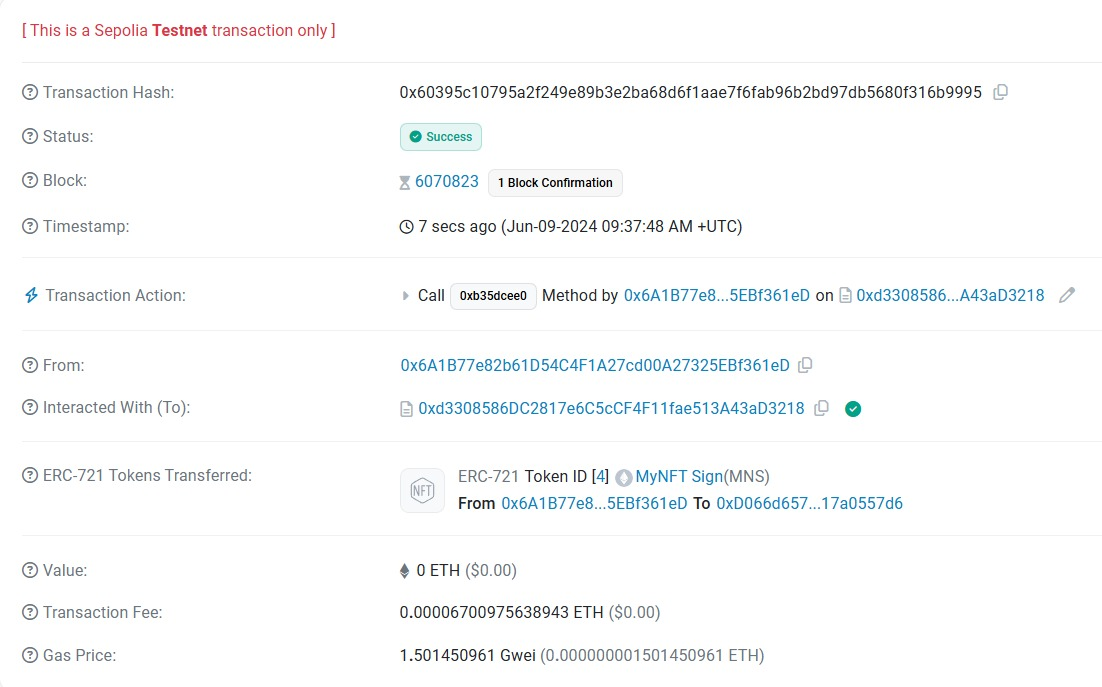
\includegraphics[scale=0.35]{gambar/detail_pada_etherscan.jpeg}}
    % Keterangan gambar yang diinputkan
    \caption{Detail pada Etherscan}
    % Label referensi dari gambar yang diinputkan
    \label{fig:detail_etherscan}
    \end{figure}

    \item pada etherscan juga terdapat detail pada NFT yang dapat dicek kepemilikannya. Jika dilihat dari gambar \ref{fig:detail_nft_etherscan} \emph{owner} dari NFT \#4 adalah \emph{address} dari \emph{user} A yang berada pada \emph{network Sepolia Ethereum Testnet}, lalu pada gambar di bawah ini setelah berhasil melakukan \emph{bridge transfer} kepemilikannya berganti kepada \emph{user} B yang berada pada \emph{network BNB Chain Testnet}.

    \begin{figure} [H] \centering
    % Nama dari file gambar yang diinputkan
    \frame{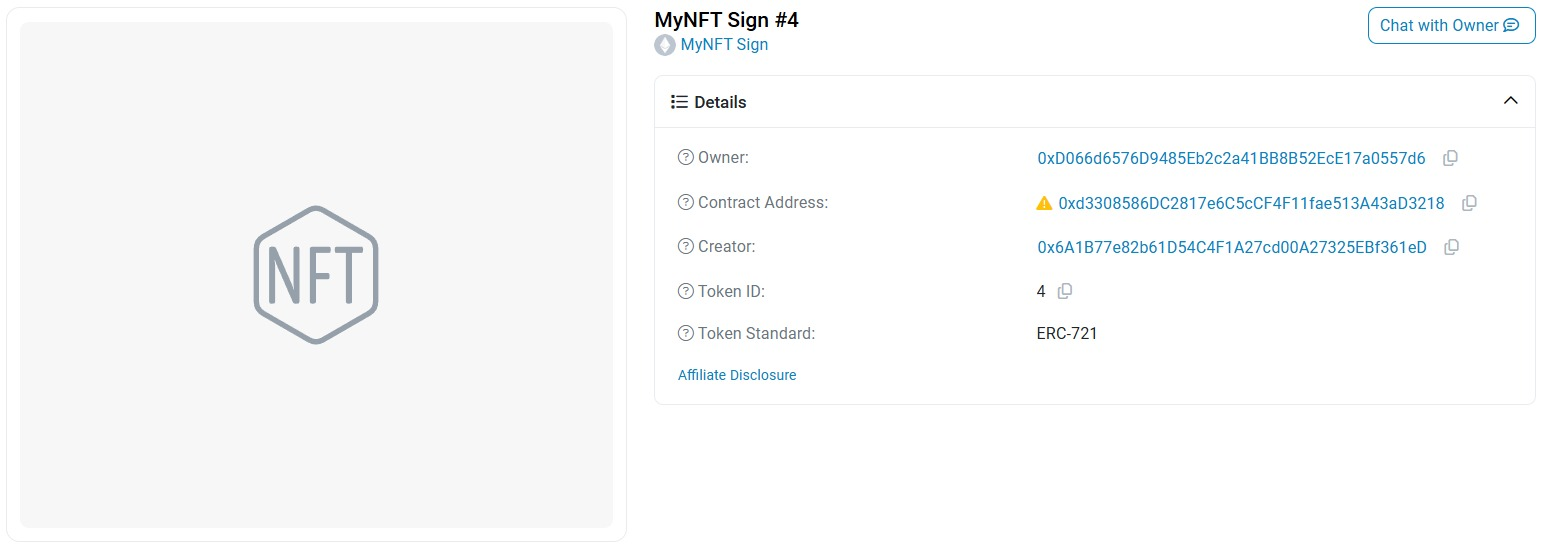
\includegraphics[scale=0.3]{gambar/nft_detail_etherscan2.jpeg}}
    % Keterangan gambar yang diinputkan
    \caption{Detail NFT pada Etherscan setelah \emph{bridge transfer}}
    % Label referensi dari gambar yang diinputkan
    \label{fig:nft_bridge_transfer}
    \end{figure}

    \item pada \emph{platform} OpenSea juga dapat dilihat pada akun milik \emph{adrress} \emph{user} B maka juga terdapat NFT yang telah terkirim ke alamatnya.

    \begin{figure} [H] \centering
    % Nama dari file gambar yang diinputkan
    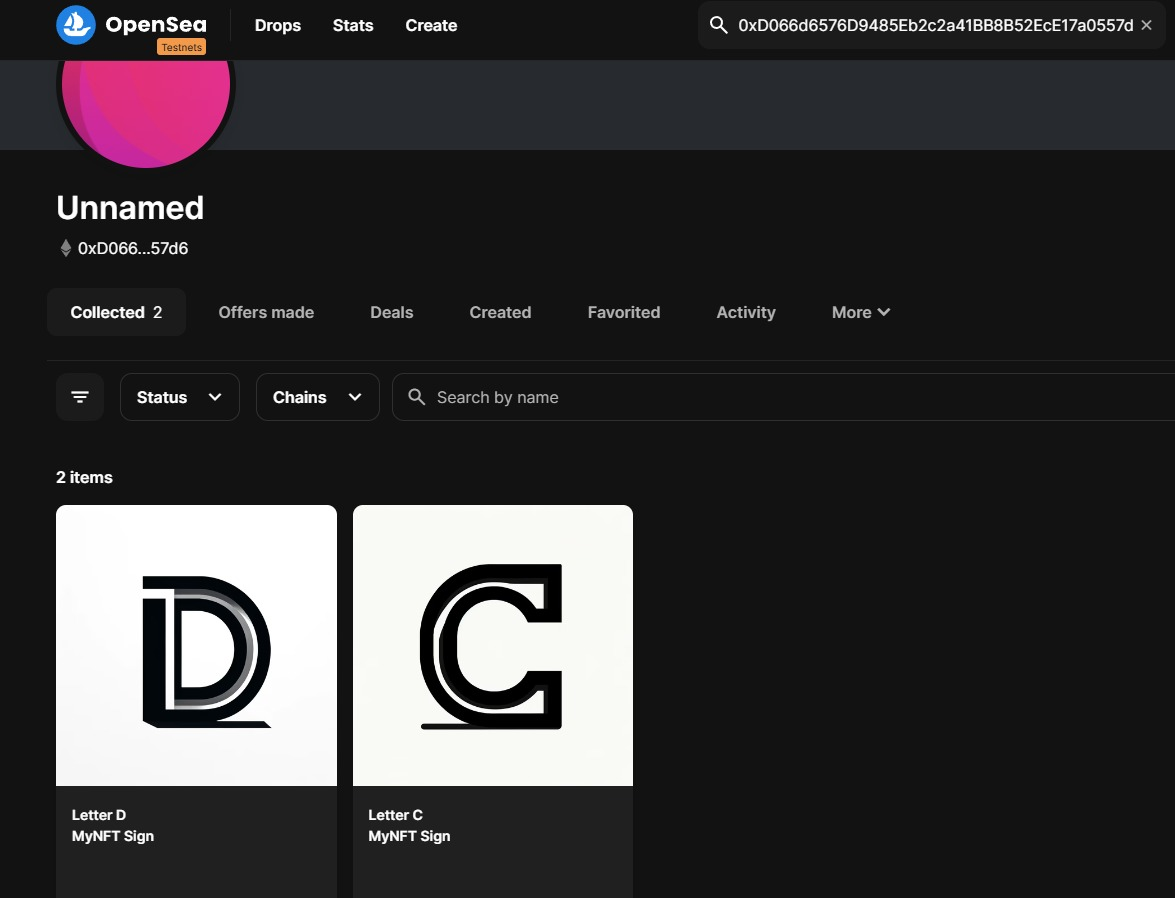
\includegraphics[scale=0.35]{gambar/nft_pada_opensea_2.jpeg}
    % Keterangan gambar yang diinputkan
    \caption{NFT pada OpenSea \emph{address} B}
    % Label referensi dari gambar yang diinputkan
    \label{fig:opensea2}
    \end{figure}
    
\end{itemize}

\subsection{Hasil Pengujian \emph{Minting} NFT}
\label{sec:pengujian_kedua}
% \begin{figure} [H] \centering
%   % Nama dari file gambar yang diinputkan
%   \frame{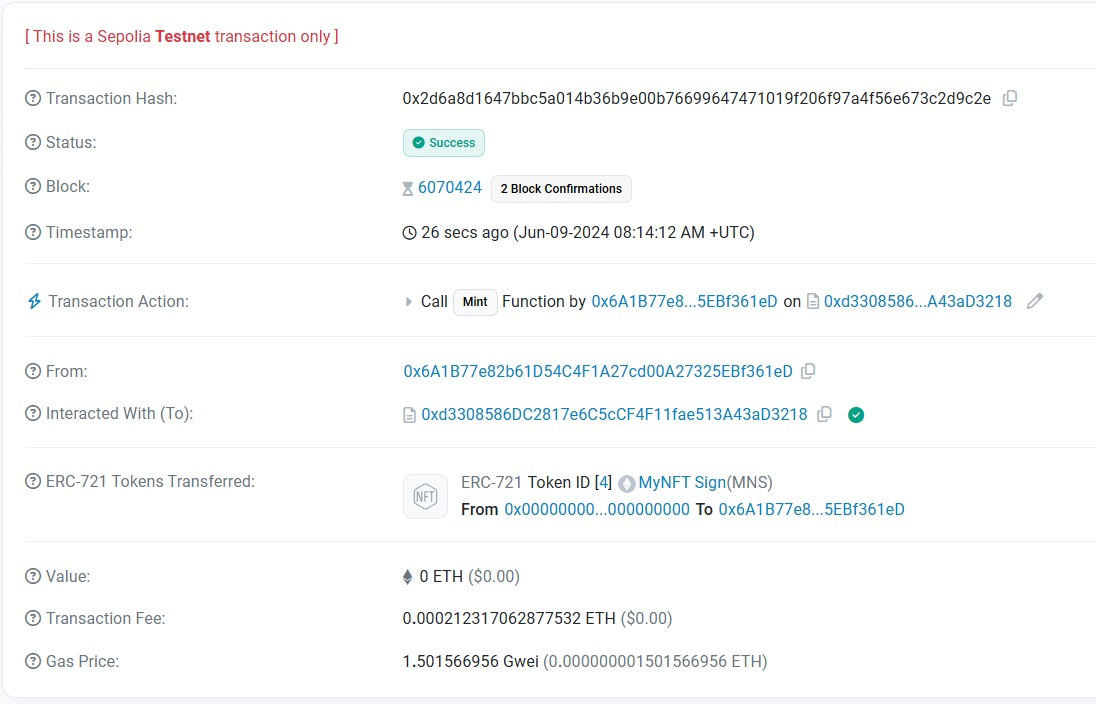
\includegraphics[scale=0.35]{gambar/detail_transaksi_etherscan.jpeg}}
%   % Keterangan gambar yang diinputkan
%   \caption{Detail transaksi \emph{minting} pada Etherscan}
%   % Label referensi dari gambar yang diinputkan
%   \label{fig:detail_transaksi}
%   \end{figure}

  \begin{longtable}[c]{|c|l|l||c|l|l|}
    \caption{Iterasi Pengujian Minting NFT}
    \label{tab:iterasi_pengujian_minting}\\
    \hline
    \textbf{No} & \textbf{Pengujian} & \textbf{Status} & \textbf{No} & \textbf{Pengujian} & \textbf{Status} \\ \hline
    \endfirsthead
    %
    \endhead
    %
    1  & Minting NFT & Success & 51 & Minting NFT & Success \\ \hline
    2  & Minting NFT & Success & 52 & Minting NFT & Success \\ \hline
    3  & Minting NFT & Success & 53 & Minting NFT & Success \\ \hline
    4  & Minting NFT & Success & 54 & Minting NFT & Success \\ \hline
    5  & Minting NFT & Success & 55 & Minting NFT & Success \\ \hline
    6  & Minting NFT & Success & 56 & Minting NFT & Success \\ \hline
    7  & Minting NFT & Success & 57 & Minting NFT & Success \\ \hline
    8  & Minting NFT & Success & 58 & Minting NFT & Success \\ \hline
    9  & Minting NFT & Success & 59 & Minting NFT & Success \\ \hline
    10 & Minting NFT & Success & 60 & Minting NFT & Success \\ \hline
    11 & Minting NFT & Success & 61 & Minting NFT & Success \\ \hline
    12 & Minting NFT & Success & 62 & Minting NFT & Success \\ \hline
    13 & Minting NFT & Success & 63 & Minting NFT & Success \\ \hline
    14 & Minting NFT & Success & 64 & Minting NFT & Success \\ \hline
    15 & Minting NFT & Success & 65 & Minting NFT & Success \\ \hline
    16 & Minting NFT & Success & 66 & Minting NFT & Success \\ \hline
    17 & Minting NFT & Success & 67 & Minting NFT & Success \\ \hline
    18 & Minting NFT & Success & 68 & Minting NFT & Success \\ \hline
    19 & Minting NFT & Success & 69 & Minting NFT & Success \\ \hline
    20 & Minting NFT & Success & 70 & Minting NFT & Success \\ \hline
    21 & Minting NFT & Success & 71 & Minting NFT & Success \\ \hline
    22 & Minting NFT & Success & 72 & Minting NFT & Success \\ \hline
    23 & Minting NFT & Success & 73 & Minting NFT & Success \\ \hline
    24 & Minting NFT & Success & 74 & Minting NFT & Success \\ \hline
    25 & Minting NFT & Success & 75 & Minting NFT & Success \\ \hline
    26 & Minting NFT & Success & 76 & Minting NFT & Success \\ \hline
    27 & Minting NFT & Success & 77 & Minting NFT & Success \\ \hline
    28 & Minting NFT & Success & 78 & Minting NFT & Success \\ \hline
    29 & Minting NFT & Success & 79 & Minting NFT & Success \\ \hline
    30 & Minting NFT & Success & 80 & Minting NFT & Success \\ \hline
    31 & Minting NFT & Success & 81 & Minting NFT & Success \\ \hline
    32 & Minting NFT & Success & 82 & Minting NFT & Success \\ \hline
    33 & Minting NFT & Success & 83 & Minting NFT & Success \\ \hline
    34 & Minting NFT & Success & 84 & Minting NFT & Success \\ \hline
    35 & Minting NFT & Success & 85 & Minting NFT & Success \\ \hline
    36 & Minting NFT & Success & 86 & Minting NFT & Success \\ \hline
    37 & Minting NFT & Success & 87 & Minting NFT & Success \\ \hline
    38 & Minting NFT & Success & 88 & Minting NFT & Success \\ \hline
    39 & Minting NFT & Success & 89 & Minting NFT & Success \\ \hline
    40 & Minting NFT & Success & 90 & Minting NFT & Success \\ \hline
    41 & Minting NFT & Success & 91 & Minting NFT & Success \\ \hline
    42 & Minting NFT & Success & 92 & Minting NFT & Success \\ \hline
    43 & Minting NFT & Success & 93 & Minting NFT & Success \\ \hline
    44 & Minting NFT & Success & 94 & Minting NFT & Success \\ \hline
    45 & Minting NFT & Success & 95 & Minting NFT & Success \\ \hline
    46 & Minting NFT & Success & 96 & Minting NFT & Success \\ \hline
    47 & Minting NFT & Success & 97 & Minting NFT & Success \\ \hline
    48 & Minting NFT & Success & 98 & Minting NFT & Success \\ \hline
    49 & Minting NFT & Success & 99 & Minting NFT & Success \\ \hline
    50 & Minting NFT & Success & 100 & Minting NFT & Success \\ \hline
    \end{longtable}

  Dari hasil pengujian yang telah dilakukan, proses minting NFT telah berhasil dijalankan sebanyak seratus kali tanpa hambatan, yang dibuktikan melalui catatan transaksi pada gambar \ref*{fig:detail_transaksi_etherscan}. Keberhasilan ini direfleksikan dan juga pada tabel \ref{tab:iterasi_pengujian_minting}, yang menunjukkan detil dari setiap transaksi yang berhasil, menegaskan keandalan dan efektivitas sistem yang dikembangkan.

  Dalam gambar yang disajikan pada gambar \ref*{fig:detail_transaksi_etherscan}, terlihat sebuah transaksi minting NFT di jaringan Sepolia Testnet yang berhasil dilakukan. Dari transaksi ini, kita dapat melihat berbagai detil penting seperti Transaction Hash, Status, Block, dan Timestamp, yang semuanya menunjukkan kesuksesan operasi tersebut. Proses minting ini dilakukan dengan menggunakan fungsi "Mint" dalam kontrak pintar, yang telah ditentukan oleh akun dengan alamat "0x6A1B77e...36b1eD" di Sepolia. Selama transaksi, ERC-721 token dengan ID 4 dipindahkan dari akun "0x000000...000000" ke akun pengguna, yang mencerminkan penciptaan dan alokasi NFT baru kepada pemiliknya. Biaya transaksi yang sangat rendah juga menyoroti efisiensi dan keefektifan penggunaan blockchain dalam pengembangan dan distribusi NFT, dengan kecepatan dan biaya yang optimal untuk operasi di jaringan testnet.

\subsection{Hasil Pengujian Transfer \emph{Ownership}}
\label{sec:pengujian_ketiga}
\begin{longtable}[c]{|c|l|l||c|l|l|}
  \caption{Iterasi Pengujian Minting NFT}
  \label{tab:iterasi_pengujian_transfer}\\
  \hline
  \textbf{No} & \textbf{Pengujian} & \textbf{Status} & \textbf{No} & \textbf{Pengujian} & \textbf{Status} \\ \hline
  \endfirsthead
  %
  \endhead
  %
  1  & Transfer Ownership & Success & 51 & Transfer Ownership & Success \\ \hline
  2  & Transfer Ownership & Success & 52 & Transfer Ownership & Success \\ \hline
  3  & Transfer Ownership & Success & 53 & Transfer Ownership & Success \\ \hline
  4  & Transfer Ownership & Success & 54 & Transfer Ownership & Success \\ \hline
  5  & Transfer Ownership & Success & 55 & Transfer Ownership & Success \\ \hline
  6  & Transfer Ownership & Success & 56 & Transfer Ownership & Success \\ \hline
  7  & Transfer Ownership & Success & 57 & Transfer Ownership & Success \\ \hline
  8  & Transfer Ownership & Success & 58 & Transfer Ownership & Success \\ \hline
  9  & Transfer Ownership & Success & 59 & Transfer Ownership & Success \\ \hline
  10 & Transfer Ownership & Success & 60 & Transfer Ownership & Success \\ \hline
  11 & Transfer Ownership & Success & 61 & Transfer Ownership & Success \\ \hline
  12 & Transfer Ownership & Success & 62 & Transfer Ownership & Success \\ \hline
  13 & Transfer Ownership & Success & 63 & Transfer Ownership & Success \\ \hline
  14 & Transfer Ownership & Success & 64 & Transfer Ownership & Success \\ \hline
  15 & Transfer Ownership & Success & 65 & Transfer Ownership & Success \\ \hline
  16 & Transfer Ownership & Success & 66 & Transfer Ownership & Success \\ \hline
  17 & Transfer Ownership & Success & 67 & Transfer Ownership & Success \\ \hline
  18 & Transfer Ownership & Success & 68 & Transfer Ownership & Success \\ \hline
  19 & Transfer Ownership & Success & 69 & Transfer Ownership & Success \\ \hline
  20 & Transfer Ownership & Success & 70 & Transfer Ownership & Success \\ \hline
  21 & Transfer Ownership & Success & 71 & Transfer Ownership & Success \\ \hline
  22 & Transfer Ownership & Success & 72 & Transfer Ownership & Success \\ \hline
  23 & Transfer Ownership & Success & 73 & Transfer Ownership & Success \\ \hline
  24 & Transfer Ownership & Success & 74 & Transfer Ownership & Success \\ \hline
  25 & Transfer Ownership & Success & 75 & Transfer Ownership & Success \\ \hline
  26 & Transfer Ownership & Success & 76 & Transfer Ownership & Success \\ \hline
  27 & Transfer Ownership & Success & 77 & Transfer Ownership & Success \\ \hline
  28 & Transfer Ownership & Success & 78 & Transfer Ownership & Success \\ \hline
  29 & Transfer Ownership & Success & 79 & Transfer Ownership & Success \\ \hline
  30 & Transfer Ownership & Success & 80 & Transfer Ownership & Success \\ \hline
  31 & Transfer Ownership & Success & 81 & Transfer Ownership & Success \\ \hline
  32 & Transfer Ownership & Success & 82 & Transfer Ownership & Success \\ \hline
  33 & Transfer Ownership & Success & 83 & Transfer Ownership & Success \\ \hline
  34 & Transfer Ownership & Success & 84 & Transfer Ownership & Success \\ \hline
  35 & Transfer Ownership & Success & 85 & Transfer Ownership & Success \\ \hline
  36 & Transfer Ownership & Success & 86 & Transfer Ownership & Success \\ \hline
  37 & Transfer Ownership & Success & 87 & Transfer Ownership & Success \\ \hline
  38 & Transfer Ownership & Success & 88 & Transfer Ownership & Success \\ \hline
  39 & Transfer Ownership & Success & 89 & Transfer Ownership & Success \\ \hline
  40 & Transfer Ownership & Success & 90 & Transfer Ownership & Success \\ \hline
  41 & Transfer Ownership & Success & 91 & Transfer Ownership & Success \\ \hline
  42 & Transfer Ownership & Success & 92 & Transfer Ownership & Success \\ \hline
  43 & Transfer Ownership & Success & 93 & Transfer Ownership & Success \\ \hline
  44 & Transfer Ownership & Success & 94 & Transfer Ownership & Success \\ \hline
  45 & Transfer Ownership & Success & 95 & Transfer Ownership & Success \\ \hline
  46 & Transfer Ownership & Success & 96 & Transfer Ownership & Success \\ \hline
  47 & Transfer Ownership & Success & 97 & Transfer Ownership & Success \\ \hline
  48 & Transfer Ownership & Success & 98 & Transfer Ownership & Success \\ \hline
  49 & Transfer Ownership & Success & 99 & Transfer Ownership & Success \\ \hline
  50 & Transfer Ownership & Success & 100 & Transfer Ownership & Success \\ \hline
  \end{longtable}  

Dari hasil pengujian yang telah dilakukan, proses transfer \emph{ownership} dari NFT telah berhasil dijalankan
sebanyak seratus kali tanpa hambatan, yang dibuktikan melalui catatan transaksi yang bisa dilihat pada gambar \ref{fig:detail_etherscan}. Keberhasilan
ini direfleksikan pada pada tabel \ref{tab:iterasi_pengujian_transfer} di bawah ini, yang menunjukkan detil dari setiap
transaksi yang berhasil, menegaskan keandalan dan efektivitas sistem yang dikembangkan. 

Dari gambar transaksi yang diberikan pada gambar \ref*{fig:detail_etherscan}, dapat dilihat bahwa NFT dengan ID 4 telah berhasil dipindahkan dari akun pengirim ke akun penerima. Detail transaksi menunjukkan bahwa tidak ada Ether (ETH) yang ditransfer sebagai bagian dari transaksi, yang menandakan bahwa proses transfer ini murni operasional tanpa melibatkan pertukaran nilai finansial. Biaya transaksi yang sangat rendah, hanya 0.000006700975683943 ETH, menegaskan efisiensi dan keekonomian proses transfer \emph{ownership} NFT ini di jaringan \emph{testnet}. \emph{Gas price} yang digunakan adalah 1.501450961 \emph{Gwei}, mengindikasikan keadaan jaringan yang optimal untuk transaksi cepat dan ekonomis. Ini mendemonstrasikan bukan hanya keandalan sistem yang dikembangkan tetapi juga potensinya untuk operasi \emph{real-time} dengan biaya minimal, sesuai dengan harapan dari penggunaan \emph{blockchain} dalam aplikasi Web 3.0.